\begin{figure}
    \begin{center}
    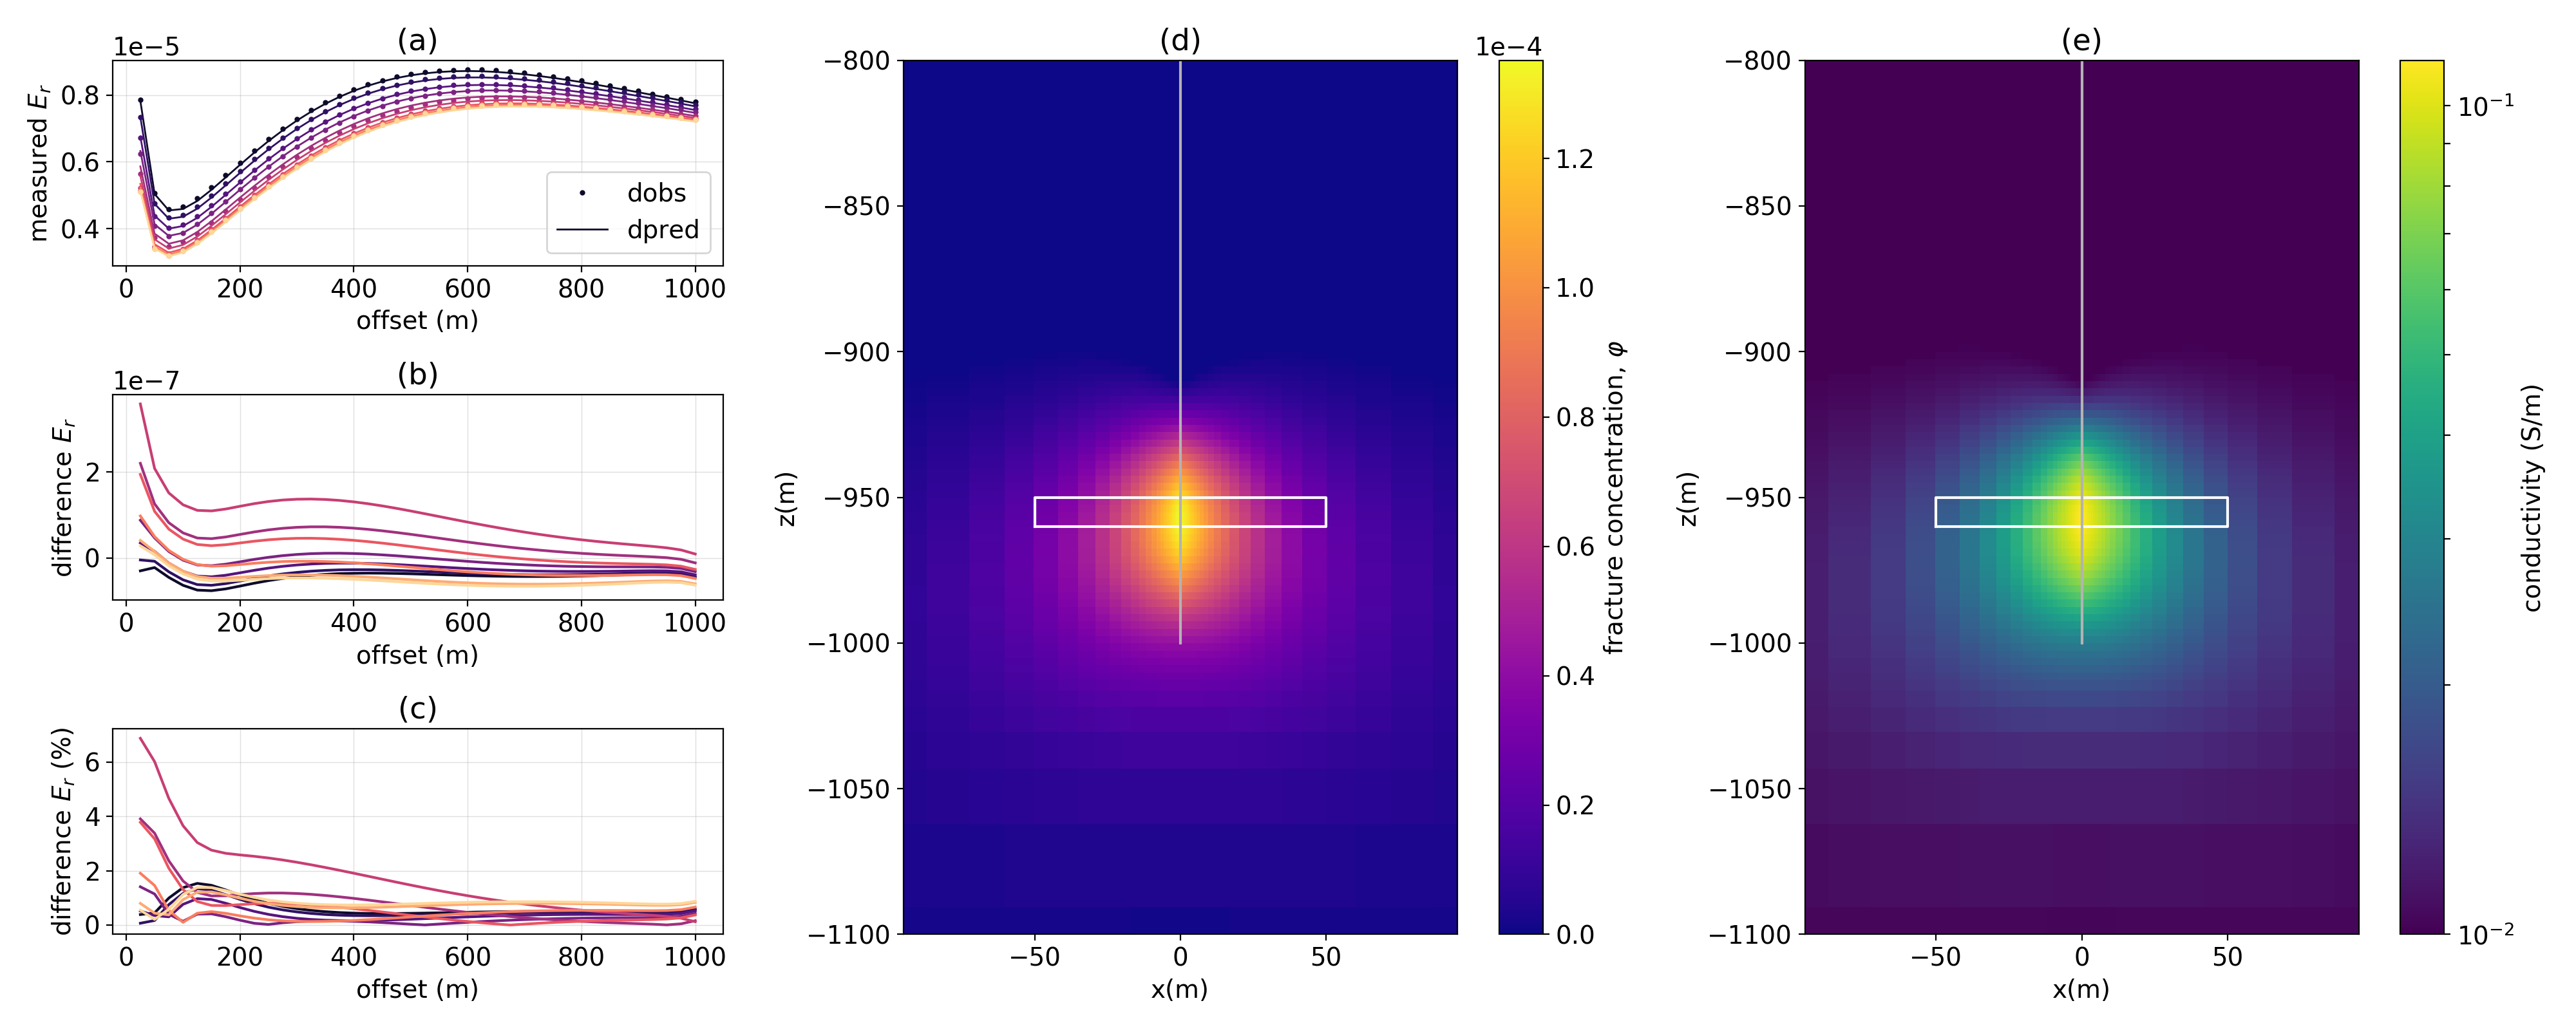
\includegraphics[width=\textwidth]{figures/inversion/dc_smooth_inversion_phi_5e-02.png}
    \end{center}
\caption{
    (a) Observed and predicted radial electric field data,
    (b) difference between the observed and predicted data (V/m),
    (c) difference between the observed and predicted data as a percentage of the observed data,
    (d) fracture concentration model, $\varphi$, recovered in the inversion, and
    (e) electrical conductivity model obtained by converting $\varphi$ to electrical conductivity using equation \ref{eq:effective_medium_theory_mapping}
    The colors in (a), (b), and (c) indicate the source location as shown in Figure \ref{fig:dc_casing_initial_data}.
    The white outline in (d) outlines the true geometry of the fracture zone and the grey line shows the location of the wellbore.
    The data are fit to a global $\chi$-factor $<$ 0.05 and the inversion took 5 iterations.
}
\label{fig:dc_smooth_inversion_phi_5e-02}
\end{figure}
